\chapter{An\'alisis Topol\'ogico de datos para Ciencia de Datos con la Libreria GUDHI}

En esta secci\'on, ilustraremos m\'etodos del ATD usando la libreria de Python
GUDHI\footnote{https://gudhi.inria.fr/python/latest} (Maria et al., 2014\cite{Maria2014})
junto con otras librerias populares como Numpy (Walt et al., 2011\cite{Walt2011}),
scikit-learn (Pedregosa et al., 2011)\cite{Pedregosa2011},
y pandas (McKinney, 2010\cite{McKinney2010}).
Esta secci\'on se enfoca en demostrar que las firmas topol\'ogicas del ATD
pueden ser facilmente calculadas y explotadas usando GUDHI.
Se pueden encontrar m\'as ejemplos en el tutorial de GUDHI en
GitHub\footnote{https://github.com/GUDHI/TDA-tutorial}.

\section{Bootstrap y Comparasi\'on de Configuraciones de Uni\'on de Prote\'inas}

Este ejemplo lo tomamos prestado de Kovacev-Nikolic et al (2016)\cite{Kovacev2016}.
En este art\'iculo, la homolog\'ia persistente es usada para analizar la uni\'on de
prote\'inas, y m\'as precisamente, compara las formas abiertas y cerradas de la
proteina de uni\'on a la maltosa (MBP), una biomol\'ecula que consiste de
$370$ residuos de amino\'acidos.
El an\'anlisis no se basa en distancias geom\'etricas en $\mathbb{R}^{3}$
sino en una m\'etrica de distancias din\'amicas definida por

\begin{equation*}
    D_{ij}=1-\cabs{C_{ij}},
\end{equation*}

donde $C$ son las matrices de correlaci\'on entre los residuos.
Los datos pueden descargarse en el siguiente
link\footnote{https://www.researchgate.net/publication/301543862\_corr}.

\begin{lstlisting}[language=Python]
import numpy as np
import gudhi as gd
import pandas as pd
import seaborn as sns

corr_protein = pd.read_csv("mypath/1anf.corr_1.txt", header=None, delim_whitespace = True)
dist_protein_1 = 1 - np.abs(corr_protein_1.values)
rips_complex_1 = gd.RipsComplex(distance_matrix = dist_protein_1, max_edge_length = 1.1)
simplex_tree_1 = rips_complex_1.create_simplex_tree(max_dimension = 2)
diag_1 = simplex_tree_1.persistence()

gd.plot_persistence_diagram(diag_1)
\end{lstlisting}

Para comparar diagramas de persistencia, usamos la distancia de cuello de botella.
El bloque a continuaci\'on calcula los intervalos de persistencia y
la distancia de cuello de botella para la $0$-homolog\'ia y $1$-homolog\'ia

\begin{lstlisting}[language=Python]
interv0_1 = simplex_tree_1.persistence_intervals_in_dimension(0)
interv0_2 = simplex_tree_2.persistence_intervals_in_dimension(0)
bot0 = gd.bottleneck_distance(interv0_1, interv0_2)

interv1_1 = simplex_tree_1.persistence_intervals_in_dimension(1)
interv1_2 = simplex_tree_2.persistence_intervals_in_dimension(1)
bot1 = gd.bottleneck_distance(interv1_1, interv1_2)
\end{lstlisting}

De esta manera, podemos calcular la matriz de distancias de cuello de botella entre las
catorce MBP. Finalmente, aplicamos metodos de reescalado multidimensional (MDS) para
encontrar la configuraci\'on en $\mathbb{R}^{2}$ que se asimile a las distancias de
cuello de botella (ver Figura \ref{fig:Figura 14}C).
Hacemos uso de la libreria scikit-learn para el MDS como sigue:

\begin{lstlisting}[language=Python]
import matplotlib.pyplot as plt
from sklearn import manifold

mds = manifold.MDS(n_components2, dissimilarity = "precomputed")
config = mds.fit(M).embedding_

plt.scatter(cong[0:7,0], config[0:7, 1], color = "red", label="closed")
plt.scatter(config[7:l,0], config[7:l, 1], color = "blue", label="red")
plt.legend(loc = 1)
\end{lstlisting}

Ahora, defnimos una banda de confianza para un diagrama usando el acercamiento
de bootstrap de cuello  de botella.
Remuestreamos sobre las lineas (y columnas) de la matriz de distancias,
y calculamos la distancia de cuello de botella entre el diagrama de persistencia original
y el diagrama de persistencia bootstrap.
Repetimos el procedimiento las veces que sean necesareas, y finalmente, estimamos el
cuantil $95\%$ de esta colecci\'on de distancias de cuello de botella.
Tomamos el valor del cuantil para definir la banda de confianza en el diagrama original
(ver Figura \ref{fig:Figura 14}D).
Sin embargo, se debe ser cuidadoso a la hora de considerar este procedimiento ya que,
hasta donde sabemos, la valides de bootstrap de cuello0 de botella no ha sido probada
en este contexto.

\section{Clasificaci\'on de Datos de Sensores}
En este experimento, la aceleraci\'on (en $3$D) de $3$ sujetos caminando
(A, B, y C) ha side monitoreada utilizando el sensor de un
smartphone\footnote{Los datos pueden ser descargados en:
http://bertrand.michel.perso.math.cnrs.fr/Enseignements/TDA/data\_acc}.
La homolog\'ia persistente no es sensible a la elecci\'on de ejes,
así que no es necesario ningun preprocesamiento de los datos para alinear
las $3$ series de tiempo a los mismos ejes.
De estas series, se escogieron aleatoriamente extractos de
$8$ segundos de la serie de tiempo completa, esto es,
$200$ puntos consecutivos de aceleraci\'on en $\mathbb{R}^{3}$.
Por cada sujeto, se extrajeron $100$ series de tiempo de esta manera.
El siguiente cloque calcula la persistencia para las filtraciones de complejos alpha para
una de las $100$ series de tiempo de la aceleraci\'on del sujeto A.

\begin{lstlisting}[language=Python]
alpha_complex_sample = gd.AlphaComplex(points = data_A_sample)
simplex_tree_sample = alpha_complex_sample.create_simplex_tree(max_alpha_square = 0.3)
diag_Alpha = simplex_tree_sample.persistence()
\end{lstlisting}

Con \verb|diag_Alpha|, podemos calcular y graficar
los paisajes de persistencia con facilidad (ver Figura \ref{fig:Figura 15}A).
Para todas las $300$ series de tiempo, calculamos los paisajes de persistencia de
dimensi\'on $0$ y $1$, y calcylamos los primeros tres paisajes de dimensi\'on $2$.
M\'as a\'un, cada paisaje de persistencia es discretizado en $1000$ puntos.
Cada serie de tiempo es entonces descrita por $6000$ variables topol\'ogicas.
Para predecir al sujeto con estas caracter\'isticas, usamos un bosque aleatorio
(Breiman, 2001\cite{Breiman2001}), ya que es eficiente cuando se maneja una
alta dimensionalidad en los datos.
Separamos nuestros datos en conjuntos de entrenamiento y prueba de manera
aleatoria varias veces.
Con esto obtenemos un error de clasificaci\'on promedio alrededor de $0.95$.
Al utilizar un modelo de bosque aleatorio, tenemos acceso a una visualizaci\'on
de las variables m\'as importantes (ver Figura\ref{fig:Figura 15}B).

\begin{figure}[ht]
    \centering
    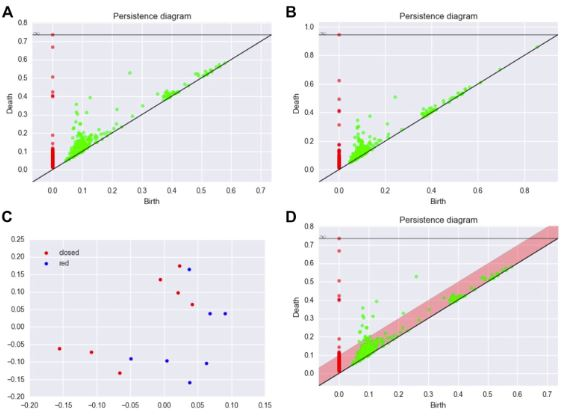
\includegraphics[width=0.85\linewidth]{./figures/Figura14.JPG}
    \caption{
        (A) Los primeros tres paisajes para la $0$-homologi\'a de la filtraci\'on alpha
        definida para una de las series de tiempo de aceleraci\'on del sujeto A.
        (B) Coeficientes de significancia de las variables del paisaje para la clasificaci\'on
        de los sujetos.
        Los primeros $3000$ coeficientes corresponden a los tres paisajes de dimensi\'on $0$
        y los \'ultimos $3000$ a los paisajes de dimensi\'on $1$.
        Hay $1000$ coeficientes por paisaje.
        N\'otese que el primer paisaje de dimensi\'on $0$ es siempre el mismo
        utilizando la filtraci\'on del complejo de Rips (un paisaje trivial), por tanto,
        loes coeficientes que le corresponden tiene un valor $0$ de significancia.
    }
    \label{fig:Figura 15}
    \vspace{15pt}
\end{figure}